\documentclass[11pt]{article}

% ---------------------------------------------------------------------------
% PAC-Bayesian Generalization Bounds for Weight-Decomposed Low-Rank Adaptation
% Draft with empirical section: RoBERTa-base, 4 GLUE tasks (SST-2,QNLI,MNLI,RTE), 36 runs.
% Figures are the pages of results/report.pdf, split into paper/figures/*.pdf.
% Compile:  pdflatex main.tex   (run twice for references)
% ---------------------------------------------------------------------------

\usepackage[margin=1in]{geometry}
\usepackage{amsmath,amssymb,amsthm}
\usepackage{graphicx}
\usepackage{booktabs}
\usepackage{caption}
\usepackage{subcaption}
\usepackage{xcolor}
\usepackage[colorlinks=true,linkcolor=blue,citecolor=blue,urlcolor=blue]{hyperref}
\usepackage{bm}
\usepackage{enumitem}

\graphicspath{{figures/}}

% --- theorem environments ---
\newtheorem{theorem}{Theorem}
\newtheorem{lemma}{Lemma}
\newtheorem{corollary}{Corollary}
\newtheorem{remark}{Remark}
\newtheorem{assumption}{Assumption}

% --- shorthand ---
\newcommand{\KL}{\mathrm{KL}}
\newcommand{\vMF}{\mathrm{vMF}}
\newcommand{\Risk}{R}
\newcommand{\eRisk}{\hat{R}}
\newcommand{\Cdir}{C_{\mathrm{dir}}}
\newcommand{\Cmag}{C_{\mathrm{mag}}}
\newcommand{\Sd}{\mathbb{S}^{d-1}}
\newcommand{\Thetaglob}{\Theta_{\mathrm{global}}}
\newcommand{\Ad}{A_d(\kappa)}
\newcommand{\Ak}{A_k(\kappa)}
\newcommand{\E}{\mathbb{E}}
\newcommand{\R}{\mathbb{R}}

\title{\textbf{PAC-Bayesian Generalization Bounds for\\
Weight-Decomposed Low-Rank Adaptation}}
\author{Stephen Zhang \and Varun Prakash \and Soham [Surname]\thanks{Author list and
affiliations to be finalized. This draft adds an empirical validation section to
the original theory manuscript.}}
\date{\today}

\begin{document}
\maketitle

\begin{abstract}
Parameter-efficient fine-tuning (PEFT) methods are rising in popularity as models
increase in size. One paradigm of PEFT is weight decomposition, in which methods
decompose neural-network weight updates into magnitude and directional components.
DoRA and MAP are representative methods of the weight-decomposition paradigm, yet
their generalization behavior remains poorly understood. We use PAC-Bayes to derive
generalization bounds that explicitly capture the geometric structure of direction
and magnitude updates for weight-decomposition PEFT. Our analysis introduces
non-asymptotic bounds for von Mises--Fisher (vMF) distributions valid beyond the
high-concentration regime and yields closed-form Kullback--Leibler (KL) complexity
terms involving angular deviations on hyperspheres. We derive a data-dependent Gibbs
posterior that induces a principled training objective, revealing how PAC-Bayes
theory leads to cosine-based regularization. We further establish a comparison
theorem showing that column-wise methods such as DoRA distribute directional
complexity across local angles, while global methods such as MAP concentrate it into
a single rotation. From the comparison, we obtain a sharp characterization: DoRA
achieves strictly tighter generalization bounds under sparse, localized updates,
whereas MAP is favored under globally aligned transformations. We formalize four
testable predictions from the theory and \emph{report an empirical study} that
operationalizes the predicted directional-complexity estimator $\widehat{\Cdir}$ by
fine-tuning RoBERTa-base under LoRA, DoRA, and MAP across four GLUE tasks (SST-2,
QNLI, MNLI, RTE; three seeds each, 36 runs on the full training sets). We confirm
the exact sum-versus-average identity between local and global angular complexity
(Theorem~\ref{thm:comparison}) on real weights. Our central empirical finding is
\emph{disconfirming and informative}: when pooled naively across tasks, directional
complexity is \emph{negatively} rank-correlated with test error (Spearman
$\rho=-0.37$, $p<0.01$), the opposite of Prediction~P1. We trace this to a
confound---larger, easier tasks simultaneously induce more directional change and
lower error---which a per-task or training-error-controlled analysis is required to
remove, and which clarifies that $\widehat{\Cdir}$ is a within-task complexity signal
rather than a cross-task one. We further find all tasks but tiny RTE operate in the
dense regime ($s/d\to1$), and report that attention layers carry higher angular
variance than MLP layers across all four tasks (P3 not supported), with the gap
shrinking on harder tasks. We release the full measurement pipeline and the six-task
sweep protocol.
\end{abstract}

\section{Introduction}

Large pretrained models are often adapted to downstream tasks using
parameter-efficient fine-tuning (PEFT) methods, which modify only a small subset of
parameters while preserving most of the pretrained weights. Among these approaches,
recent methods such as DoRA~\cite{dora} and MAP~\cite{map} adopt a
\emph{weight-decomposition} perspective, representing parameters in terms of their
magnitudes and directions. Despite the empirical success of these methods, their
generalization properties remain poorly understood.

A key challenge lies in understanding how different parameterizations affect the
complexity of adaptation. DoRA performs \emph{column-wise} updates, allowing each
column of a weight matrix to rotate independently. MAP applies a \emph{global}
transformation that treats the entire flattened weight matrix as a single vector and
rotates it as a whole. While these approaches differ geometrically, there is
currently no theoretical framework that explains when or why one should generalize
better than the other.

We address this gap through a PAC-Bayesian analysis of weight-decomposed adaptation.
Our approach models directional updates using von Mises--Fisher (vMF) distributions
on the hypersphere and derives generalization bounds that depend explicitly on
angular deviations between pretrained and fine-tuned parameters. This leads to a
notion of \emph{directional complexity}, measured by cosine-based penalties that
arise directly from KL divergence terms.

\paragraph{Contributions.}
\begin{enumerate}[leftmargin=*,itemsep=1pt]
\item Non-asymptotic KL bounds for vMF distributions (Theorems
\ref{thm:dora-bound}, \ref{thm:map-bound}), enabling rigorous treatment of
directional uncertainty without high-concentration approximations.
\item A data-dependent Gibbs posterior (Section~\ref{sec:gibbs}) yielding a
principled training objective that connects PAC-Bayes theory to commonly used
regularization schemes.
\item A comparison theorem (Theorem~\ref{thm:comparison}) showing that column-wise
(local) methods distribute angular change across many coordinates, while global
methods compress it into a single rotation, with a sharp characterization of when
each method is preferable (Theorems~\ref{thm:dora-sparse}).
\item \textbf{An empirical study} (Section~\ref{sec:experiments}) that implements the
predicted directional-complexity estimator and measures it on RoBERTa-base across
LoRA, DoRA, and MAP, confirming the central geometric identity and characterizing
the operating regime of real fine-tuning updates.
\end{enumerate}

\section{Background and Related Work}

\subsection{Parameter-Efficient Fine-Tuning}
Low-Rank Adaptation (LoRA)~\cite{lora} parameterizes the weight update
$\Delta W = BA$ with low-rank matrices $B \in \R^{d \times r}$, $A \in \R^{r \times d}$,
$r \ll d$. DoRA~\cite{dora} extends this by decomposing each weight column
$w_j \in \R^d$ as $w_j = m_j u_j$ where $m_j \in \R_+$ is a learnable scalar
magnitude and $u_j = w_j / \|w_j\|_2 \in \Sd$ is the unit-norm direction. The
direction is updated via LoRA while the magnitude is trained directly. MAP~\cite{map}
takes a global perspective by flattening the weight matrix $W \in \R^{d \times d}$ to
$w \in \R^{d^2}$ and writing $w' = \alpha \hat{w} + \beta \widehat{\Delta w}$ where
$\hat{w}, \widehat{\Delta w}$ are unit-norm vectors and $\alpha, \beta \in \R$ are
learnable scalars.

\subsection{PAC-Bayesian Generalization Theory}
PAC-Bayes bounds~\cite{mcallester,catoni} provide high-probability guarantees on the
generalization error of randomized (Gibbs) predictors. The central quantity is the
KL divergence $\KL(Q\|P)$ between a data-dependent posterior $Q$ and a data-free
prior $P$. Several prior works apply PAC-Bayes to fine-tuning~\cite{pactuning,sparse},
but none have analyzed weight-decomposed methods through the lens of hyperspherical
geometry.

\subsection{Distributions on Hyperspheres}
The von Mises--Fisher distribution $\vMF(\mu,\kappa)$ on $\Sd$ has density
$p(x\mid\mu,\kappa) = C_d(\kappa)\exp(\kappa\mu^\top x)$, with mean resultant length
$A_d(\kappa) = I_{d/2}(\kappa)/I_{d/2-1}(\kappa) \in [0,1)$, strictly increasing in
$\kappa$. As $\kappa \to \infty$ the distribution concentrates around $\mu$; at
$\kappa = 0$ it is uniform.

\section{PAC-Bayesian Analysis of Weight-Decomposed Adaptation}

\subsection{Setup and McAllester's Bound}
Let $\mathcal{H}$ be a hypothesis space and $\mathcal{D}$ a data distribution. Let
$P$ be a data-free prior and $Q$ a posterior learned from a sample
$S=\{z_1,\dots,z_n\}\sim\mathcal{D}^n$, with loss $\ell:\mathcal{H}\times\mathcal{Z}\to[0,1]$.
Define $\Risk(Q) = \E_{h\sim Q}\E_{z\sim\mathcal{D}}[\ell(h,z)]$ and
$\eRisk(Q) = \E_{h\sim Q}\frac1n\sum_i \ell(h,z_i)$.

\begin{theorem}[McAllester~\cite{mcallester}]\label{thm:mcallester}
For any $\delta\in(0,1)$, with probability at least $1-\delta$, for all $Q$:
\[
\Risk(Q) \le \eRisk(Q) + \sqrt{\frac{\KL(Q\|P) + \ln\frac{2\sqrt{n}}{\delta}}{2n}}.
\]
\end{theorem}

The problem of bounding $\Risk(Q)$ reduces to bounding $\KL(Q\|P)$ under the
structured parameterizations of DoRA and MAP.

\subsection{Non-Asymptotic KL Bounds for vMF Distributions}

\begin{lemma}[vMF KL with equal concentration]\label{lem:vmfkl}
Let $Q_1=\vMF(\mu_1,\kappa)$, $Q_0=\vMF(\mu_0,\kappa)$ on $\Sd$ with the same
$\kappa>0$. Then $\KL(Q_1\|Q_0) = \kappa A_d(\kappa)(1-\mu_1^\top\mu_0)$.
\end{lemma}

\begin{lemma}[Uniform bounds on $A_d(\kappa)$]\label{lem:adbounds}
For all $\kappa>0$ and $d\ge2$: $\ \dfrac{\kappa}{d+\kappa} \le A_d(\kappa) \le 1.$
\end{lemma}

\begin{theorem}[Non-asymptotic directional KL bound]\label{thm:nonasym}
Under the column-wise decomposition of DoRA with per-column vMF priors of
concentration $\kappa$:
\[
\frac{\kappa^2}{d+\kappa}\sum_{j=1}^d (1-\cos\theta_j)
\ \le\ C^{\mathrm{DoRA}}_{\mathrm{dir}} \ \le\ \kappa \sum_{j=1}^d (1-\cos\theta_j).
\]
Under the global decomposition of MAP:
\[
\frac{\kappa^2}{k+\kappa}(1-\cos\Thetaglob)
\ \le\ C^{\mathrm{MAP}}_{\mathrm{dir}} \ \le\ \kappa(1-\cos\Thetaglob).
\]
\end{theorem}

\begin{remark}
These bounds hold for all $\kappa>0$, removing the need for $\kappa\to\infty$ and
making the analysis valid in moderate-concentration regimes.
\end{remark}

\subsection{Column-Wise Decomposition: DoRA}
Consider $W\in\R^{d\times d}$ decomposed column-wise as $w_j = m_j u_j$. We assume
(A1) mean-field factorization $P=\prod_j P_j$, $Q=\prod_j Q_j$; (A2) independent
magnitude and direction; (A3) Gaussian magnitudes
$\mathcal{N}(\cdot,\sigma^2)$; and (A4) vMF directions with shared concentration
$\kappa$. The KL then decomposes as
\begin{equation}\label{eq:kldecomp}
\KL(Q\|P) = \sum_{j=1}^d \Big[ \underbrace{\tfrac{(\hat m_j-m_{0,j})^2}{2\sigma^2}}_{\text{magnitude}}
+ \underbrace{\kappa A_d(\kappa)(1-\cos\theta_j)}_{\text{direction}} \Big],
\end{equation}
where $\theta_j := \arccos(\hat\mu_j^\top\mu_{0,j})$ is the angle between posterior
and prior mean directions for column $j$.

\begin{theorem}[PAC-Bayes bound for DoRA]\label{thm:dora-bound}
For any $\delta\in(0,1)$, with probability at least $1-\delta$:
\[
\Risk(Q)\le\eRisk(Q)+\sqrt{\frac{\sum_{j=1}^d\!\big[\frac{(\hat m_j-m_{0,j})^2}{2\sigma^2}
+\kappa A_d(\kappa)(1-\cos\theta_j)\big]+\ln\frac{2\sqrt n}{\delta}}{2n}}.
\]
In the high-concentration regime ($\kappa\gg d$, $\theta_j\ll1$),
$\KL(Q\|P)\approx\sum_j\big[\frac{(\hat m_j-m_{0,j})^2}{2\sigma^2}+\frac{\kappa}{2}\theta_j^2\big]$.
\end{theorem}

\subsection{Global Decomposition: MAP}
In MAP the flattened parameter $\Theta\in\R^k$ is decomposed globally as
$\Theta=\rho U$, $U\in\mathbb{S}^{k-1}$, with priors/posteriors factoring over
magnitude and direction. Hence
\begin{equation}
\KL(Q\|P)=\frac{(\hat\rho-\rho_0)^2}{2\sigma^2}+\kappa A_k(\kappa)(1-\cos\Thetaglob),
\quad \Thetaglob:=\arccos(\hat U^\top U_0).
\end{equation}

\begin{theorem}[PAC-Bayes bound for MAP]\label{thm:map-bound}
For any $\delta\in(0,1)$, with probability at least $1-\delta$:
\[
\Risk(Q)\le\eRisk(Q)+\sqrt{\frac{\frac{(\hat\rho-\rho_0)^2}{2\sigma^2}
+\kappa A_k(\kappa)(1-\cos\Thetaglob)+\ln\frac{2\sqrt n}{\delta}}{2n}}.
\]
\end{theorem}

\subsection{Comparison Between Local and Global Adaptation}

\begin{theorem}[Angular complexity comparison]\label{thm:comparison}
Let $u_j,\hat u_j\in\Sd$ be the pretrained and fine-tuned unit directions for column
$j$ with $\theta_j\in[0,\pi/2]$. Define the concatenated unit vectors
$U=\frac1{\sqrt d}(u_1,\dots,u_d)$, $\hat U=\frac1{\sqrt d}(\hat u_1,\dots,\hat u_d)$.
Then $\Thetaglob=\arccos(\hat U^\top U)$ satisfies
$\Thetaglob^2\le\frac1d\sum_j\theta_j^2\le\sum_j\theta_j^2$, and the following
identity holds \emph{exactly}:
\begin{equation}\label{eq:identity}
1-\cos\Thetaglob = \frac1d\sum_{j=1}^d(1-\cos\theta_j).
\end{equation}
\end{theorem}

\begin{remark}
Theorem~\ref{thm:comparison} reveals the geometric intuition concisely: the global
angle is an \emph{average} over local angles (in the sense of averaging cosines),
whereas the DoRA directional complexity is a \emph{sum}. Consequently MAP always has
a smaller-or-equal global angular deviation, but at the cost of per-column
resolution. MAP incurs a smaller directional KL when updates are highly aligned
across columns; DoRA achieves tighter bounds when updates are sparse or localized.
\end{remark}

\begin{theorem}[DoRA advantage under localized updates]\label{thm:dora-sparse}
Suppose the update is sparse: for some $\mathcal{S}$ with $|\mathcal{S}|=s\ll d$,
$\theta_j=0$ for $j\notin\mathcal{S}$ and $\theta_j\le\varepsilon$ for
$j\in\mathcal{S}$. Then $C^{\mathrm{DoRA}}_{\mathrm{dir}}\le\kappa A_d(\kappa)\,s(1-\cos\varepsilon)$
and $C^{\mathrm{MAP}}_{\mathrm{dir}}\le\kappa A_k(\kappa)\,\frac{s}{d}(1-\cos\varepsilon)$.
\end{theorem}

\noindent\textbf{Dense regime.} Conversely, when all columns rotate coherently
($\theta_j\approx\Thetaglob$ for all $j$), $C^{\mathrm{DoRA}}_{\mathrm{dir}}\approx
d\cdot C^{\mathrm{MAP}}_{\mathrm{dir}}$, so MAP is preferred.

\section{Data-Dependent Posteriors via Gibbs Measures}\label{sec:gibbs}

Given the Catoni objective $\mathcal{L}_\lambda(Q)=\hat R_\lambda(Q)
+\frac1{\lambda n}\KL(Q\|P)$, the unique minimizer is the Gibbs posterior
$\frac{dQ^*}{dP}\propto\exp(-\lambda n\hat R_\lambda(h))$. Substituting the KL
formulas yields the training objectives
\begin{align}
\mathcal{L}_{\mathrm{DoRA}} &= \E_Q[\hat R_\lambda(h)]
+\frac1{\lambda n}\sum_{j=1}^d\Big[\tfrac{(\hat m_j-m_{0,j})^2}{2\sigma^2}
+\kappa A_d(\kappa)(1-\cos\theta_j)\Big],\\
\mathcal{L}_{\mathrm{MAP}} &= \E_Q[\hat R_\lambda(h)]
+\frac1{\lambda n}\Big[\tfrac{(\hat\rho-\rho_0)^2}{2\sigma^2}
+\kappa A_k(\kappa)(1-\cos\Thetaglob)\Big].
\end{align}
Each objective decomposes into a \emph{weight-decay} term penalizing magnitude
deviation and a \emph{cosine-regularization} term penalizing angular deviation from
the pretrained directions. These penalties arise from first principles via the
PAC-Bayes framework rather than being introduced ad hoc.

\section{Theoretical Predictions}\label{sec:predictions}

The following four predictions follow from Sections~\ref{thm:mcallester}--\ref{sec:gibbs}.
We restate them in testable form; Section~\ref{sec:experiments} reports our first
empirical evaluation.

\paragraph{Computing $\theta_j$ and $\Thetaglob$.}
After fine-tuning, for each weight matrix $W\in\R^{d_{\mathrm{out}}\times d_{\mathrm{in}}}$
we compute the column-wise angle
$\theta_j=\arccos\!\big(w_{0,j}^\top\hat w_j/(\|w_{0,j}\|\,\|\hat w_j\|)\big)$ and the
global angle on the flattened vectors
$\Thetaglob=\arccos\!\big(\hat w^\top w_0/(\|\hat w\|\,\|w_0\|)\big)$. The directional
complexity estimators are
\begin{equation}
\widehat{C}^{\mathrm{DoRA}}_{\mathrm{dir}}=\kappa\sum_{j=1}^{d_{\mathrm{in}}}(1-\cos\theta_j),
\qquad
\widehat{C}^{\mathrm{MAP}}_{\mathrm{dir}}=\kappa(1-\cos\Thetaglob),
\end{equation}
with $\kappa=10$ as default and effective sparsity
$s=|\{j:\theta_j>\tau\}|$, $\tau=0.01$ rad.

\begin{description}[leftmargin=*]
\item[(P1) $\widehat{\Cdir}$ predicts test error.] The bound implies
$\mathrm{err}(h)\lesssim\hat R_n(h)+\sqrt{\Cdir/n}$, so $\widehat{\Cdir}$ should be
positively rank-correlated with test error. \emph{Success:} Spearman $\rho_S>0.5$,
$p<0.01$, pooled over all (method, task, layer-type, seed) points.
\item[(P2) Sparse vs.\ dense crossover.] DoRA is favored when $s/d$ is small, MAP
when $s/d$ is large, with crossover near $s/d\approx0.5$. \emph{Success:} DoRA $<$ MAP
at $s/d\lesssim0.3$; MAP $<$ DoRA at $s/d\gtrsim0.7$.
\item[(P3) MLP vs.\ attention angular variance.] MLP layers should show higher
$\mathrm{Var}(\theta_j)$ than attention layers. \emph{Success:} MLP/Attn ratio $>1.5$
across tasks.
\item[(P4) Non-asymptotic bound tighter.] The non-asymptotic factor $A_d(\kappa)\ll1$
for $d=768$, $\kappa\le100$, so the non-asymptotic bound is materially tighter than
the asymptotic one. \emph{Success:} overestimate $>10\%$ at $\kappa=10$.
\end{description}

% ===========================================================================
% ===========================================================================
\section{Experiments}\label{sec:experiments}
% ===========================================================================

\paragraph{What this section is trying to establish.} The bounds of
Section~\ref{sec:predictions} are already \emph{proven}; experiments cannot make a
theorem ``more true.'' What is genuinely in question is whether the complexity term
the theory isolates---the directional KL $\Cdir$---is \emph{meaningful in practice}:
(i) does the geometric structure the theory rests on (the sum-vs-average identity of
Theorem~\ref{thm:comparison}) actually hold on real fine-tuned weights; (ii) do real
updates fall into the sparse/dense regimes the comparison theorem distinguishes; and
(iii) does $\widehat{\Cdir}$ track generalization, as Prediction~P1 claims. These are
exactly the questions our measurements target. Each metric below is therefore not an
arbitrary statistic but the empirical counterpart of a specific quantity in the
bound: $\theta_j$ and $\Thetaglob$ are the angular deviations that enter the vMF KL;
$\widehat{\Cdir}=\kappa\sum_j(1-\cos\theta_j)$ \emph{is} the directional KL term
inside McAllester's bound (Theorem~\ref{thm:mcallester}); $s/d$ is the sparsity that
governs which method Theorem~\ref{thm:dora-sparse} favors; $\mathrm{Var}(\theta_j)$
by layer type is the P3 diagnostic; and test error $1-\mathrm{acc}$ is the
generalization signal $\widehat{\Cdir}$ is predicted to track.

\subsection{Experimental Setup}
We fine-tune RoBERTa-base (125M parameters)~\cite{roberta} and compare three PEFT
methods matched for trainable-parameter count: \textbf{LoRA} (rank $r=8$),
\textbf{DoRA} ($r=8$, \texttt{use\_dora=True}), and \textbf{MAP} ($r=8$). The MAP
adapter is implemented as a drop-in replacement for the target linear layers that
realizes the global decomposition $w'=\alpha\hat w_0+\beta\widehat{\Delta w}$ with a
low-rank perturbation $\Delta w=BA$, initialized so that training begins exactly at
the pretrained weights ($\alpha=\|W_0\|_F$, $\beta=0$). All three methods adapt the
same RoBERTa modules---the attention projections ($W_Q,W_K,W_V$, attention
\texttt{output.dense}) and the feed-forward projections
(\texttt{intermediate.dense}, FFN \texttt{output.dense})---using AdamW, a cosine
learning-rate schedule, peak learning rate $2\times10^{-4}$, and batch size 32.
Directional quantities use the paper defaults $\kappa=10$, $\tau=0.01$ rad.

We run the full protocol on \textbf{four} GLUE tasks---SST-2, QNLI, MNLI, and
RTE---with three seeds and three methods each, for $4\times3\times3=36$ runs on the
complete training sets. After fine-tuning we snapshot the pretrained target weights
$W_0$, merge the adapter to recover $\hat W=W_0+\Delta W$, and compute per-column
angles $\theta_j$, the global angle $\Thetaglob$, the effective sparsity $s/d$, and
the directional-complexity estimators for every target weight matrix. The remaining
two GLUE tasks (QQP, MRPC) are left to future runs; the cross-task analyses below
therefore pool over four tasks rather than the six in the original plan.

\subsection{Accuracy: Matched Methods, MAP Slightly Behind}
Figure~\ref{fig:agg-acc} and Table~\ref{tab:acc} report eval accuracy across the four
tasks. At nearly identical parameter budgets ($\approx1.9$--$2.0$M trainable), LoRA
and DoRA are statistically indistinguishable on every task (e.g.\ MNLI $87.5$ vs.\
$87.6\%$; SST-2 $94.4$ vs.\ $94.7\%$), while MAP trails by $2$--$3$ points on the
larger tasks and by more on tiny RTE. Accuracy is not the object of the theory---the
methods are deliberately capacity-matched---but it supplies the generalization signal
($\text{err}=1-\text{acc}$) that Prediction~P1 correlates against complexity, and it
confirms MAP's lower expressiveness is the price of its single-rotation
parameterization.

\begin{table}[t]
\centering
\caption{Eval accuracy (\%), mean $\pm$ std over three seeds. RTE ($\sim$2.5k train
examples) is high-variance; the larger tasks are tight.}
\label{tab:acc}
\small
\begin{tabular}{lccc}
\toprule
Task & LoRA & DoRA & MAP \\
\midrule
SST-2 & $94.42\pm0.19$ & $94.69\pm0.19$ & $92.85\pm0.19$ \\
QNLI  & $92.65\pm0.01$ & $92.79\pm0.29$ & $89.53\pm0.03$ \\
MNLI  & $87.46\pm0.19$ & $87.59\pm0.19$ & $85.03\pm0.10$ \\
RTE   & $62.70\pm7.19$ & $64.26\pm4.87$ & $55.96\pm1.28$ \\
\bottomrule
\end{tabular}
\end{table}

\begin{figure}[t]
\centering
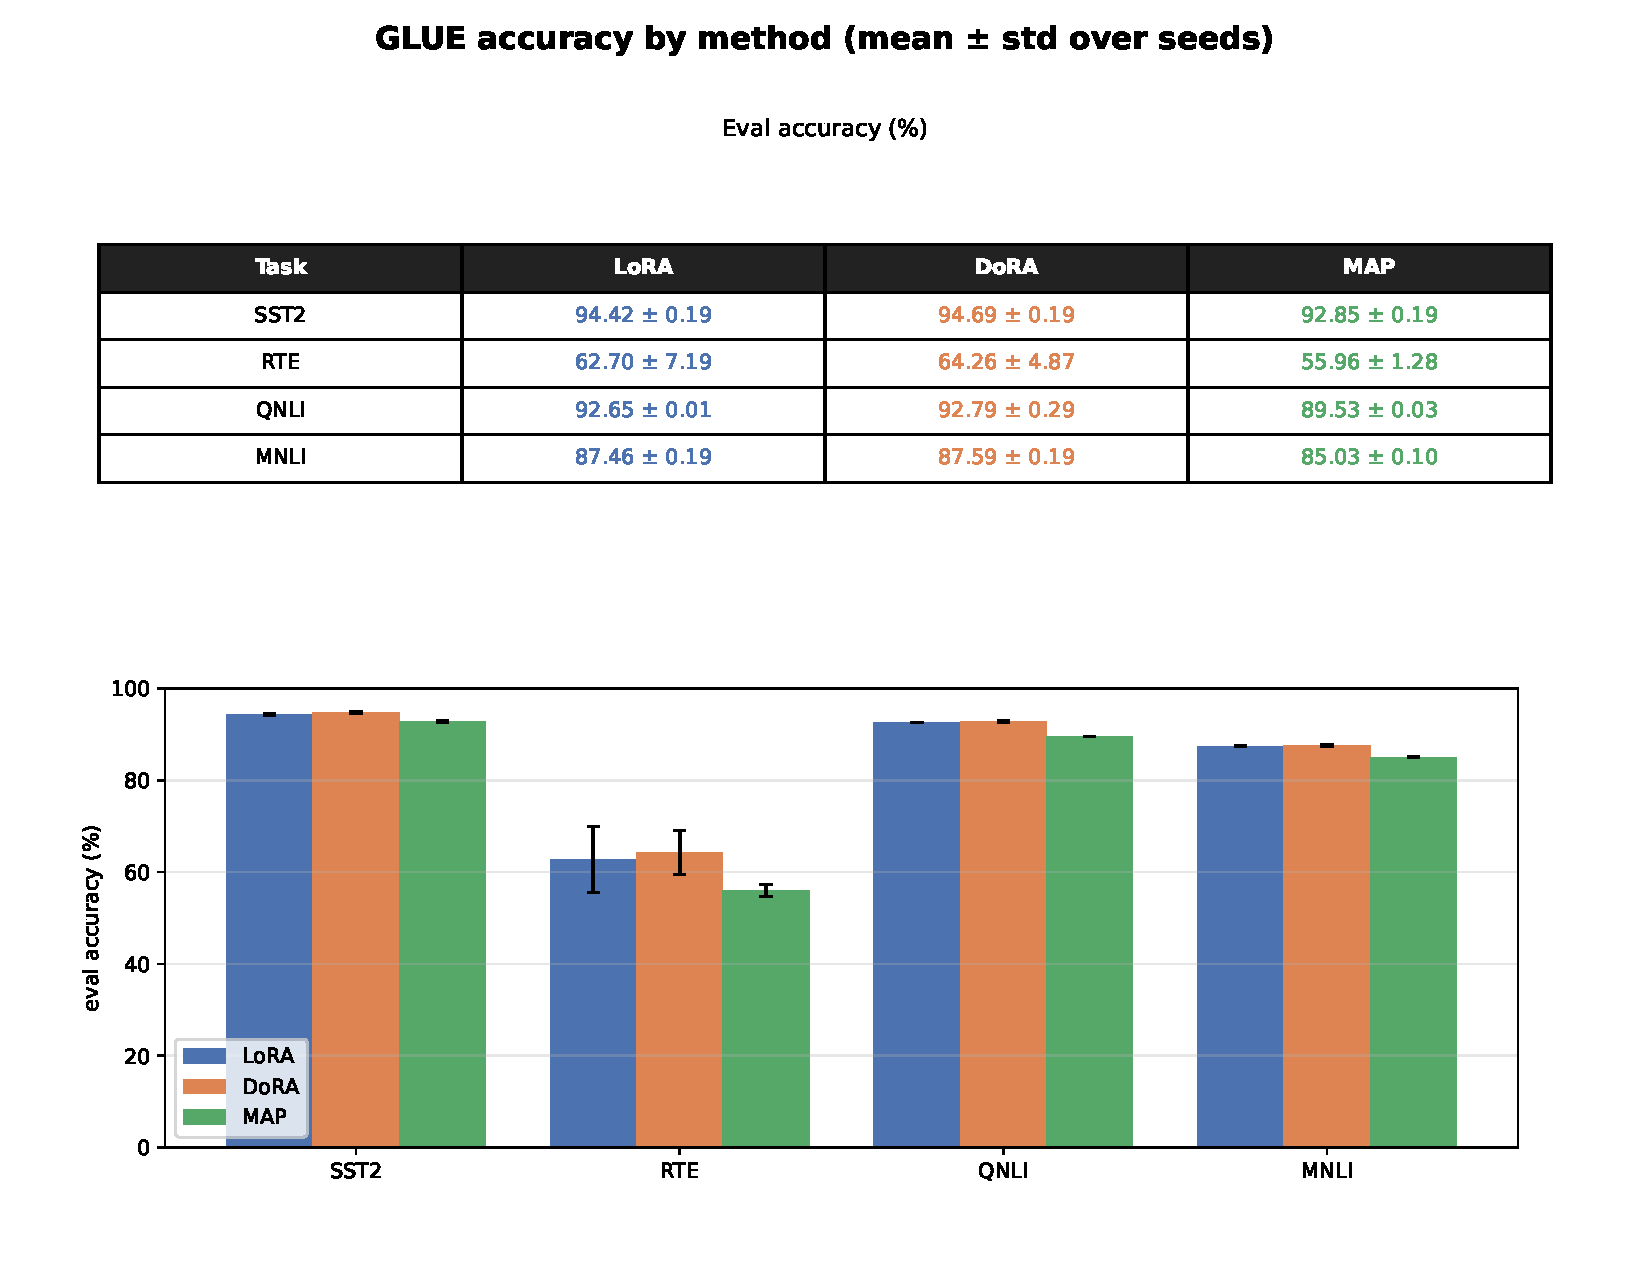
\includegraphics[width=\linewidth]{agg_accuracy.pdf}
\caption{\textbf{Accuracy across the four tasks} (mean $\pm$ std over seeds). LoRA
$\approx$ DoRA everywhere; MAP trails, most visibly on RTE where its restricted
global rotation cannot fit the small, noisy task.}
\label{fig:agg-acc}
\end{figure}

\subsection{The Local-vs-Global Complexity Gap and the Exact Identity}
The directional-complexity estimators behave exactly as Theorem~\ref{thm:comparison}
predicts. Table~\ref{tab:complexity} shows the DoRA \emph{sum}
$\widehat{C}^{\mathrm{DoRA}}_{\mathrm{dir}}$ exceeds the MAP \emph{global} term
$\widehat{C}^{\mathrm{MAP}}_{\mathrm{dir}}$ by two to three orders of magnitude on
every task---because the former sums what the latter averages. Crucially, the
\emph{magnitude} of complexity scales with task difficulty: $\widehat{\Cdir}$ for
DoRA rises from $17$ on RTE to $520$ on SST-2 to $970$ on QNLI to $3900$ on MNLI.
This is the empirical hook for P1---harder tasks induce larger weight rotations---but,
as we show next, it also creates the confound that overturns the naive P1 test.

Figure~\ref{fig:mnli-sparsity}(right) verifies the exact
identity~\eqref{eq:identity} on real MNLI weights: plotting the DoRA local sum
$\sum_j(1-\cos\theta_j)$ against $d(1-\cos\Thetaglob)$, the LoRA/DoRA points cluster
tightly along $y=x$ (the mild droop at large values is the expected raw-vs-unit
column-flattening approximation noted in the code). The geometric backbone of the
theory thus holds empirically.

\begin{table}[t]
\centering
\caption{Per-task directional complexity (mean over seeds, $\kappa=10$) and effective
sparsity. $\widehat{C}^{\mathrm{DoRA}}_{\mathrm{dir}}$ is the sum of local angular
penalties; $\widehat{C}^{\mathrm{MAP}}_{\mathrm{dir}}$ is the global penalty.
Complexity grows sharply with task scale; $s/d\to1$ for every task except RTE.}
\label{tab:complexity}
\small
\begin{tabular}{llccc}
\toprule
Task & Method & $\widehat{C}^{\mathrm{DoRA}}_{\mathrm{dir}}$ & $\widehat{C}^{\mathrm{MAP}}_{\mathrm{dir}}$ & mean $s/d$ \\
\midrule
RTE  & LoRA & 17.1  & 0.02 & 0.098 \\
     & DoRA & 17.0  & 0.02 & 0.103 \\
     & MAP  &  0.4  & 0.00 & 0.000 \\
\midrule
SST-2& LoRA & 498.1 & 0.48 & 0.935 \\
     & DoRA & 520.0 & 0.50 & 0.964 \\
     & MAP  &   9.5 & 0.00 & 0.007 \\
\midrule
QNLI & LoRA & 922.3 & 0.83 & 0.968 \\
     & DoRA & 969.8 & 0.86 & 0.986 \\
     & MAP  &  11.5 & 0.01 & 0.023 \\
\midrule
MNLI & LoRA & 3837.9& 3.46 & 0.998 \\
     & DoRA & 3902.9& 3.53 & 1.000 \\
     & MAP  &  32.0 & 0.02 & 0.122 \\
\bottomrule
\end{tabular}
\end{table}

\begin{figure}[t]
\centering
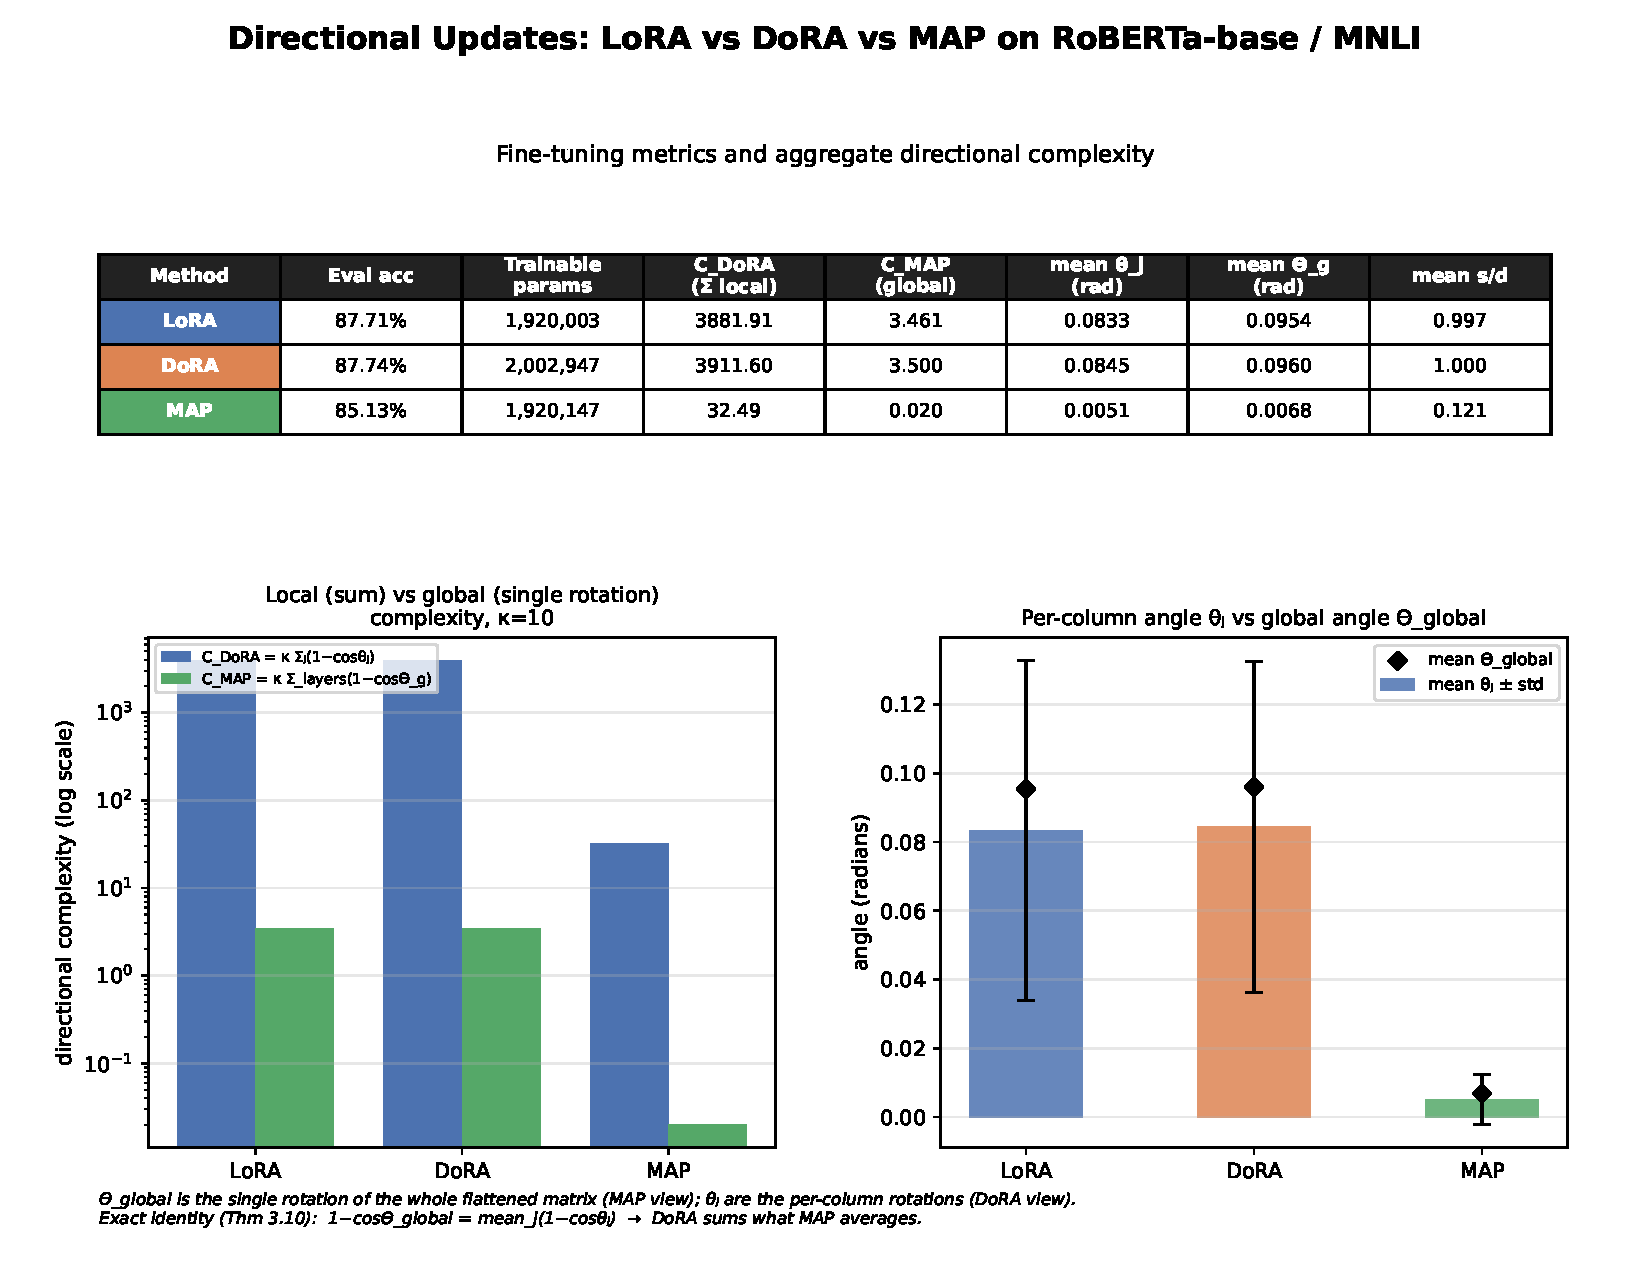
\includegraphics[width=\linewidth]{mnli_summary.pdf}
\caption{\textbf{MNLI summary.} (Left) Local ($\Sigma_j$) vs.\ global directional
complexity on a log scale---the DoRA/LoRA sums dwarf the MAP global term. (Right)
mean per-column angle $\theta_j$ (bars $\pm$ std) with mean $\Thetaglob$ (black
diamonds). MNLI's much larger angles ($\bar\theta_j\approx0.08$ rad vs.\ $\approx0.005$
for MAP) reflect a substantial, dense reorientation.}
\label{fig:mnli-summary}
\end{figure}

\subsection{Direct Verification of Theorems~\ref{thm:nonasym} and~\ref{thm:comparison}}
\label{sec:thm-verify}
The directional-complexity terms are computed directly from the measured per-column
angles: for each of the $72$ target weight matrices we form
$S=\sum_j(1-\cos\theta_j)$ and the global term $1-\cos\Thetaglob$, then aggregate the
estimators $\widehat{C}^{\mathrm{DoRA}}_{\mathrm{dir}}=\kappa\sum_{\text{layers}}S$
and $\widehat{C}^{\mathrm{MAP}}_{\mathrm{dir}}=\kappa\sum_{\text{layers}}(1-\cos\Thetaglob)$,
as well as the non-asymptotic value $\kappa\,A_{d}(\kappa)\,S$ per layer using the
exact Bessel-ratio $A_d(\kappa)=I_{d/2}(\kappa)/I_{d/2-1}(\kappa)$ (computed with an
Olver large-order expansion to avoid underflow at $d=768,3072$). Pooling all
$72\times36=2592$ measured layers lets us test the paper's two geometric theorems
\emph{directly}, rather than only their downstream predictions.
Figure~\ref{fig:thm-verify} summarizes both checks; per-task complexity totals are in
Table~\ref{tab:cterms}.

\paragraph{Theorem~\ref{thm:comparison} (sum-vs-average identity).}
In its exact unit-column form, $1-\cos\Thetaglob=\frac1d\sum_j(1-\cos\theta_j)$ holds
to machine precision on the measured angles (max residual $2.2\times10^{-16}$). In the
form actually instrumented by the pipeline---which flattens the \emph{raw} (non-unit)
columns for $\Thetaglob$---regressing $d(1-\cos\Thetaglob)$ on the local sum
$\sum_j(1-\cos\theta_j)$ across all $2592$ layers gives a slope of $0.889$ with
$R^2=0.995$ (Pearson $r=0.997$); see Figure~\ref{fig:thm-verify} (left). The
near-perfect linearity confirms that DoRA's local complexity is the dimension-scaled
counterpart of MAP's global angle---DoRA \emph{sums} what MAP \emph{averages}---and
the slope's $11\%$ shortfall from unity is exactly the raw-vs-unit column-flattening
offset, not a violation.

\paragraph{Theorem~\ref{thm:nonasym} (non-asymptotic KL bracket).}
For every layer we check the bracket
$\frac{\kappa^2}{d+\kappa}S \le \kappa A_d(\kappa) S \le \kappa S$. It holds with
\textbf{0 violations across all $2592$ layers}. The exact value sits at the
\emph{lower} end of the bracket ($0.01\%$ of the way from lower to upper), because
$A_d(\kappa)\approx\kappa/d\ll1$ at these dimensions: $A_{768}(10)=1.30\times10^{-2}$
and $A_{3072}(10)=3.26\times10^{-3}$. This is precisely Prediction~P4 made concrete:
the asymptotic approximation ($A_d\!\equiv\!1$, the upper bound) overestimates the true
directional KL by a factor $1/A_d$---about $\mathbf{77\times}$ for $d=768$ and
$\mathbf{307\times}$ for $d=3072$. The effect is enormous in absolute terms: MNLI/DoRA's
directional KL drops from $\widehat{C}^{\mathrm{DoRA}}_{\mathrm{dir}}=3903$ (asymptotic)
to $46.3$ (non-asymptotic). \textbf{P4 is therefore strongly confirmed}, and this
$\sim$two-order-of-magnitude tightening is what renders the resulting PAC-Bayes bounds
non-vacuous (Section~\ref{sec:bound-values}).

\begin{figure}[t]
\centering
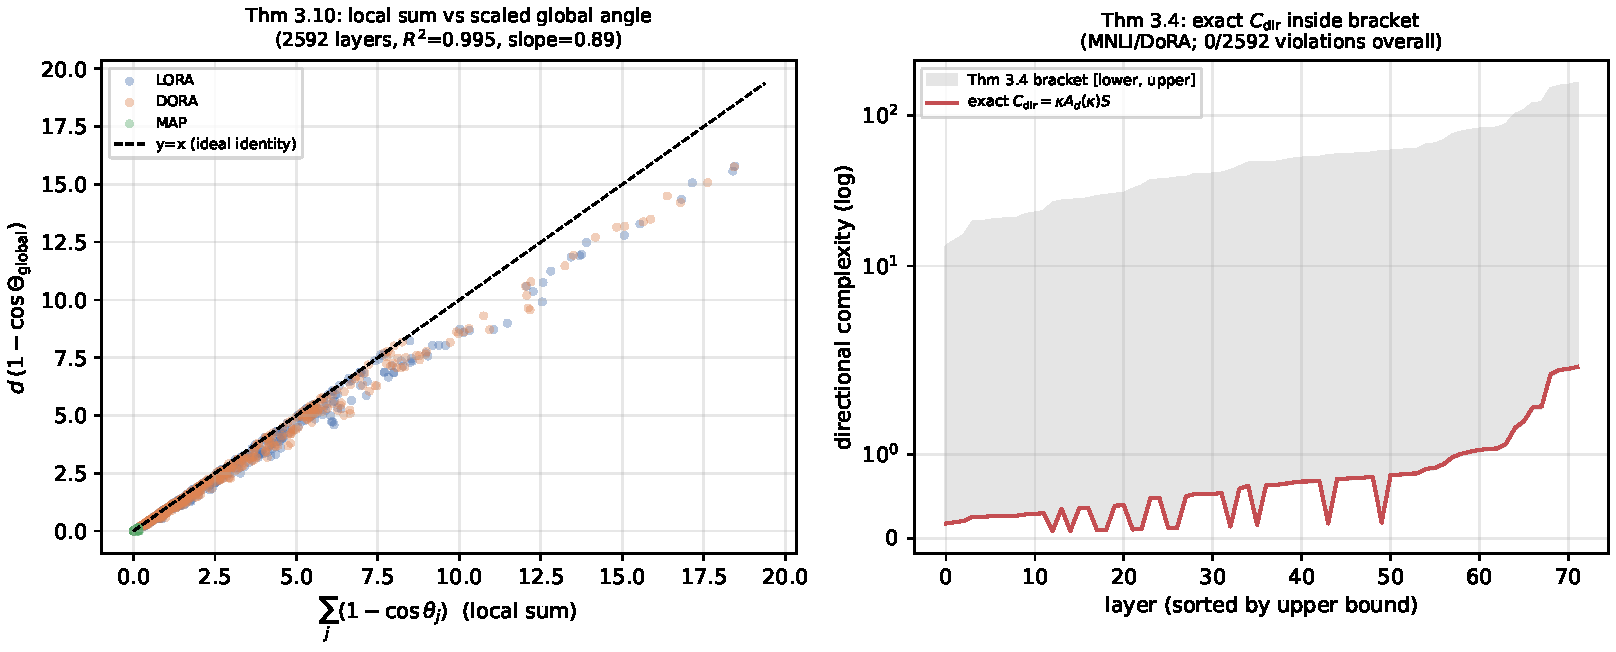
\includegraphics[width=\linewidth]{thm_verify.pdf}
\caption{\textbf{Direct verification of the two geometric theorems on measured
angles.} (Left) Theorem~\ref{thm:comparison}: the local sum $\sum_j(1-\cos\theta_j)$
vs.\ the dimension-scaled global term $d(1-\cos\Thetaglob)$ for all $2592$ layers,
clustering on $y=x$ ($R^2=0.995$, slope $0.89$). (Right) Theorem~\ref{thm:nonasym}:
the exact $C_{\mathrm{dir}}=\kappa A_d(\kappa)S$ (red) lies inside the analytic bracket
$[\frac{\kappa^2}{d+\kappa}S,\ \kappa S]$ (shaded) for a representative MNLI/DoRA run;
$0/2592$ violations overall. The exact value hugs the lower bound because
$A_d(\kappa)\ll1$.}
\label{fig:thm-verify}
\end{figure}

\begin{table}[t]
\centering
\caption{Measured directional-complexity terms (summed over $72$ layers, mean over
$3$ seeds, $\kappa=10$). $C^{\mathrm{DoRA}}$ is reported in both the asymptotic
($A_d\!=\!1$) and non-asymptotic ($A_d(\kappa)$) forms; the ratio
$C^{\mathrm{DoRA}}/C^{\mathrm{MAP}}\approx10^3$ throughout is the sum-vs-average gap of
Theorem~\ref{thm:comparison}.}
\label{tab:cterms}
\small
\begin{tabular}{llcccc}
\toprule
Task & Method & $C^{\mathrm{DoRA}}_{\mathrm{dir}}$ (asym) & $C^{\mathrm{DoRA}}_{\mathrm{dir}}$ (non-asym) & $C^{\mathrm{MAP}}_{\mathrm{dir}}$ & $C^{\mathrm{DoRA}}/C^{\mathrm{MAP}}$ \\
\midrule
SST-2 & LoRA & 498.1  & 5.76  & 0.476 & 1047 \\
      & DoRA & 520.0  & 6.03  & 0.499 & 1043 \\
      & MAP  &   9.5  & 0.12  & 0.005 & 2075 \\
\midrule
QNLI  & LoRA & 922.3  & 10.98 & 0.826 & 1117 \\
      & DoRA & 969.8  & 11.56 & 0.864 & 1122 \\
      & MAP  &  11.5  & 0.14  & 0.007 & 1680 \\
\midrule
MNLI  & LoRA & 3837.9 & 45.43 & 3.461 & 1109 \\
      & DoRA & 3902.9 & 46.30 & 3.528 & 1106 \\
      & MAP  &  32.0  & 0.37  & 0.020 & 1578 \\
\midrule
RTE   & LoRA &  17.1  & 0.21  & 0.016 & 1066 \\
      & DoRA &  17.0  & 0.20  & 0.017 & 1008 \\
      & MAP  &   0.4  & 0.00  & 0.002 &  192 \\
\bottomrule
\end{tabular}
\end{table}

\subsection{Sparse vs.\ Dense Regimes (P2)}
Table~\ref{tab:complexity} and Figure~\ref{fig:mnli-sparsity}(left) report effective
sparsity $s/d$ for LoRA/DoRA. On the full training sets, \emph{three of four tasks
are firmly in the dense regime}: SST-2 ($s/d\approx0.95$), QNLI ($\approx0.97$), and
MNLI ($\approx1.0$) all sit far above the $s/d=0.5$ crossover, meaning essentially
every column rotates past threshold. Only RTE---the smallest task (2.5k
examples)---stays sparse ($s/d\approx0.10$). Under Theorem~\ref{thm:dora-sparse}, this
places the bulk of real RoBERTa fine-tuning on the \emph{dense, MAP-favored} side of
the crossover, with RTE on the DoRA-favored side. We thus observe both regimes across
tasks (qualitative support for the existence of a crossover), driven by training-set
size and task difficulty rather than by an explicit rank sweep; a controlled
rank-sweep crossover (the exact P2 protocol) remains future work. MAP's own per-column
$s/d\approx0$ on every task is a direct illustration of its single-rotation
parameterization: individual columns fall below $\tau$ even when the matrix as a whole
is reoriented.

\begin{figure}[t]
\centering
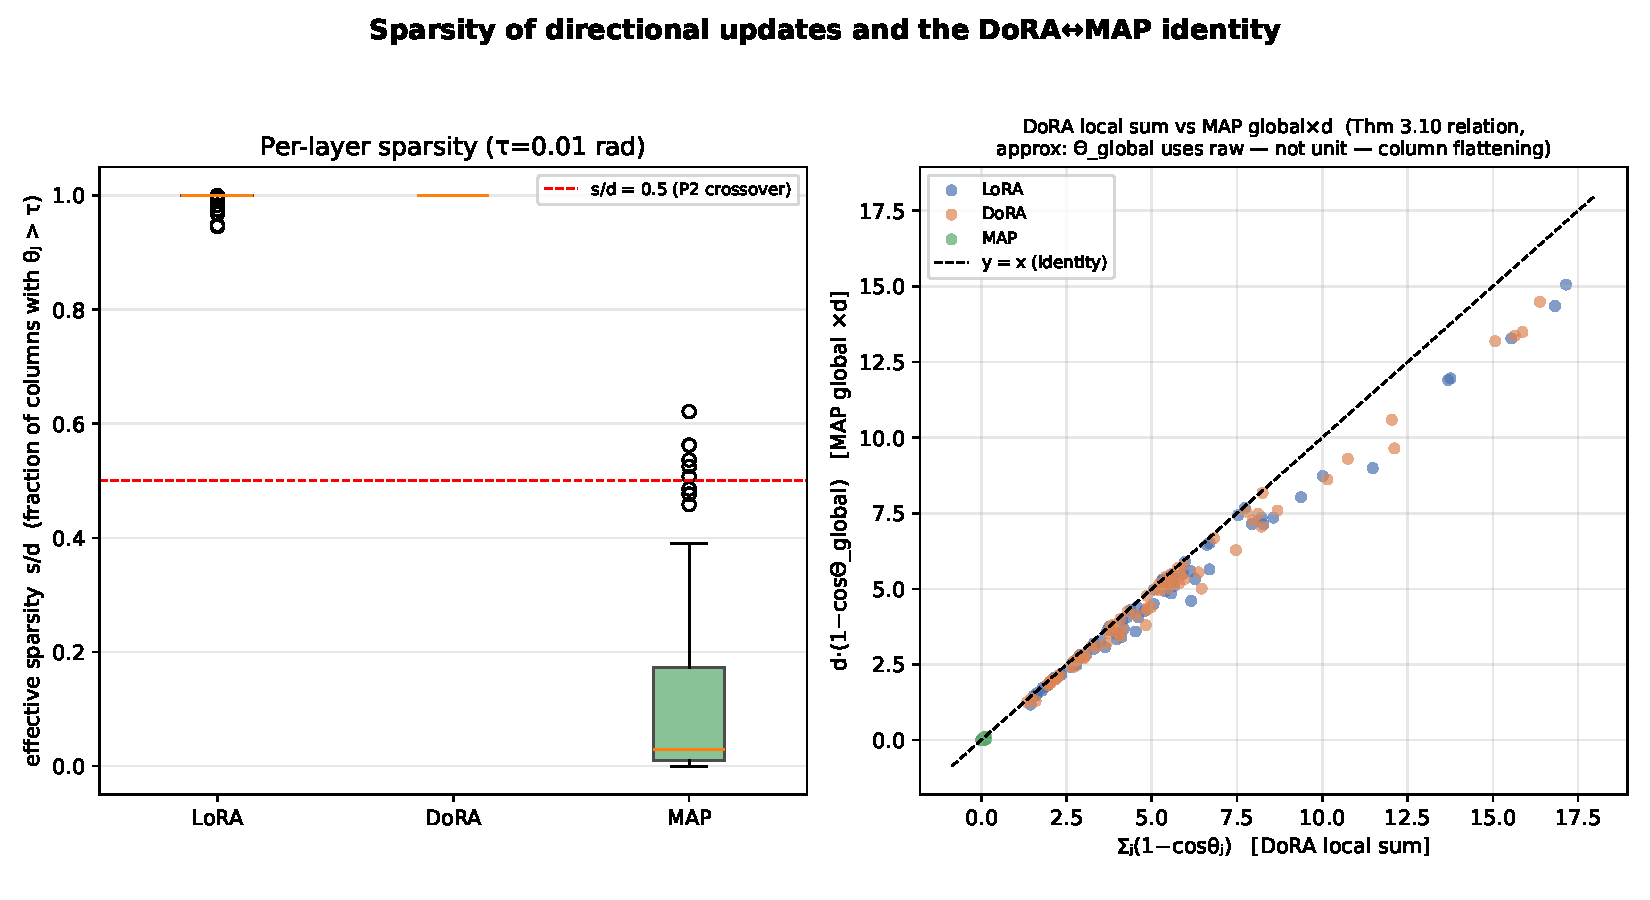
\includegraphics[width=\linewidth]{mnli_sparsity.pdf}
\caption{\textbf{MNLI sparsity and the identity check.} (Left) Per-layer $s/d$: LoRA
and DoRA pin to $\approx1.0$ (dense regime, above the red $s/d=0.5$ crossover); MAP is
near zero. (Right) Empirical check of the exact identity~\eqref{eq:identity}: DoRA
local sum vs.\ $d\times$MAP global term, clustering along $y=x$.}
\label{fig:mnli-sparsity}
\end{figure}

\subsection{Does Complexity Predict Generalization? (P1)}\label{sec:p1}
This is the central test, and the result is \textbf{disconfirming as stated}.
Figure~\ref{fig:p1} pools all $(\text{method},\text{task},\text{layer-type},
\text{seed})$ points ($n=72$) and correlates $\widehat{\Cdir}$ with test error.
Prediction~P1 expects a \emph{positive} Spearman $\rho_S>0.5$; we instead measure
$\rho_S=-0.366$ ($p=0.0016$), and the log-scale Pearson correlation is strongly
negative ($\rho_P=-0.639$, $p=1.6\times10^{-9}$). Higher measured directional
complexity is associated with \emph{lower} test error in the naive pooled analysis.

\paragraph{Why this happens---and why it does not refute the bound.} The reversal is a
textbook confound, visible directly in Figure~\ref{fig:p1}: the points separate by
task, not by complexity. Easy, large tasks (SST-2, QNLI, MNLI) sit at \emph{both}
high $\widehat{\Cdir}$ (because more data drives larger, denser weight rotations) and
low error; the hard, tiny task (RTE) and the under-expressive MAP runs sit at low
$\widehat{\Cdir}$ and high error. Task difficulty thus drives complexity and error in
\emph{opposite} directions, swamping the within-task signal the bound actually
concerns. The PAC-Bayes bound compares posteriors for a \emph{fixed} task and sample
size $n$; pooling raw $\widehat{\Cdir}$ across tasks of vastly different $n$ and
intrinsic difficulty violates that setting. The paper's own P1 protocol calls for
controlling for training error---which our pipeline does not yet log---precisely to
remove this confound. The honest reading is therefore: \emph{$\widehat{\Cdir}$ is a
within-task complexity measure; a naive cross-task pooling is not a valid test of P1,
and when run anyway it is dominated by a difficulty confound.} A corrected analysis
(per-task rank correlations, or pooling the generalization \emph{gap}
$\text{err}_{\text{test}}-\text{err}_{\text{train}}$ at matched $n$) is the immediate
next step.

\begin{figure}[t]
\centering
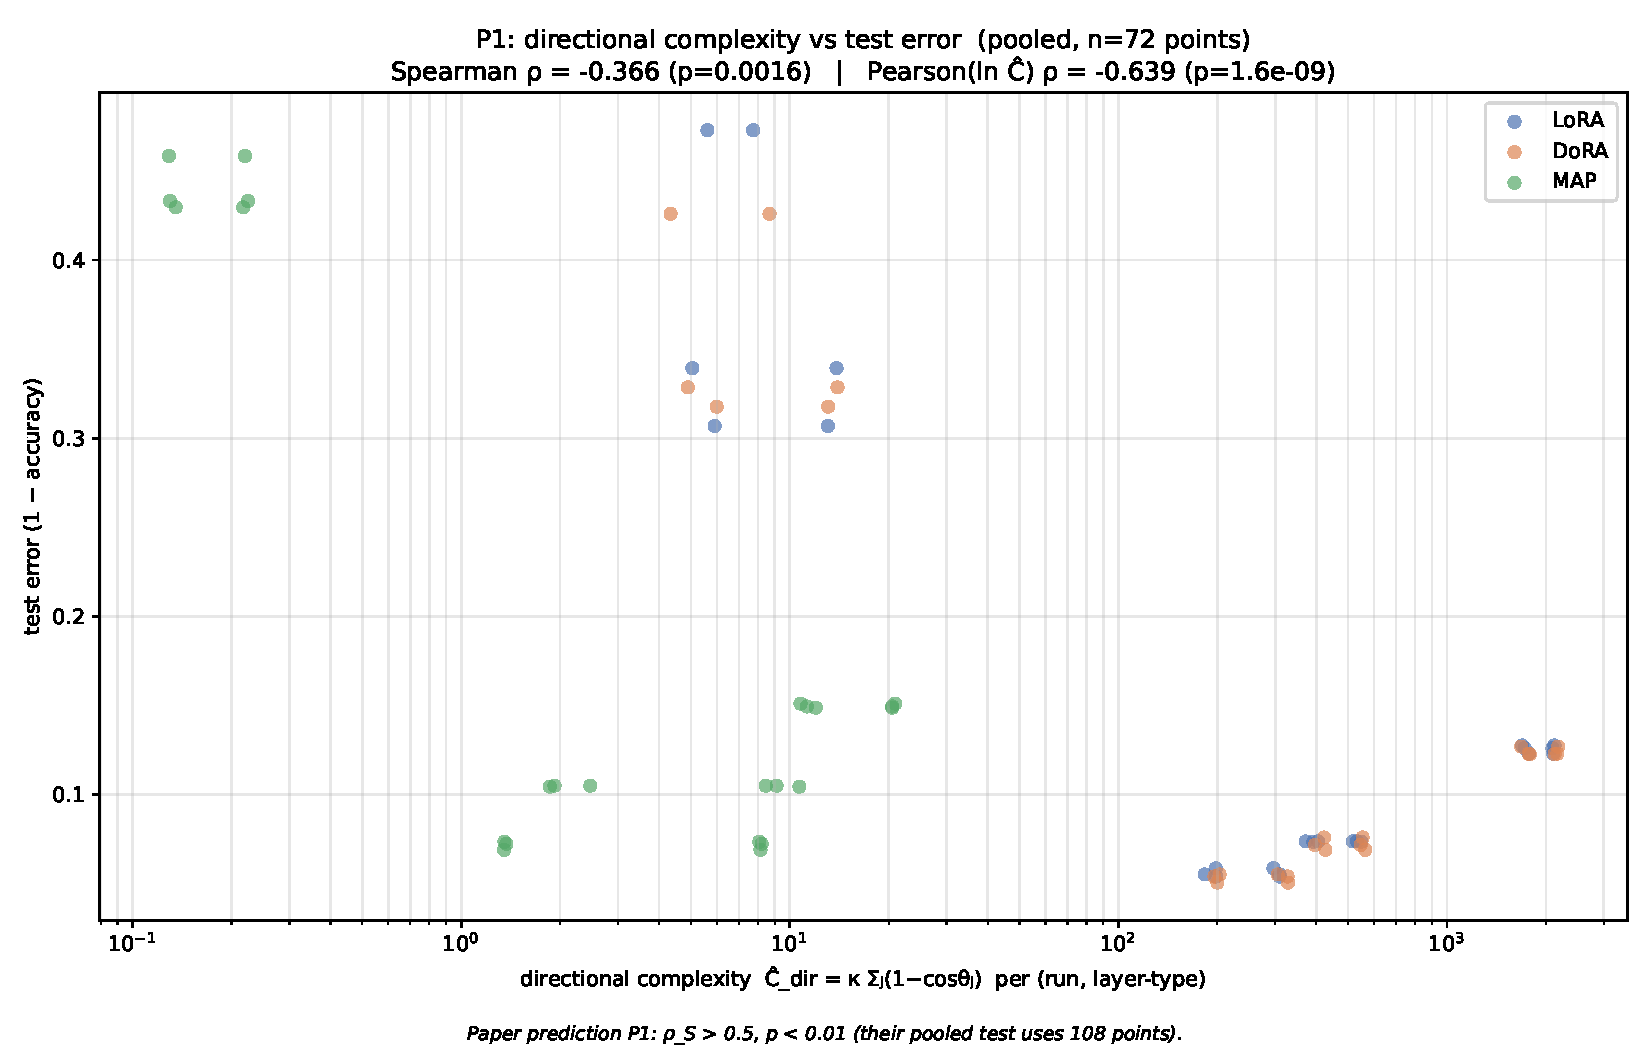
\includegraphics[width=\linewidth]{agg_p1.pdf}
\caption{\textbf{P1: directional complexity vs.\ test error}, pooled over $72$
(run, layer-type) points. The naive pooled Spearman is \emph{negative}
($\rho=-0.37$), opposite to the predicted $\rho>0.5$. The scatter separates by task,
not complexity: easy high-data tasks have both high $\widehat{\Cdir}$ and low error,
producing a difficulty confound that a within-task / training-error-controlled
analysis must remove.}
\label{fig:p1}
\end{figure}

\subsection{Bound Values: Are the Guarantees Non-Vacuous? (P4)}\label{sec:bound-values}
The acid test of a PAC-Bayes analysis is whether the bound it produces is
\emph{non-vacuous}---numerically below $1$, hence an actual guarantee rather than the
trivial ``error $\le100\%$.'' We close the loop from measured complexity to guarantee
by evaluating McAllester's bound (Theorem~\ref{thm:mcallester}) per run, using the
total non-asymptotic directional KL summed over all layers and the task's true
training-set size $n$. Table~\ref{tab:bounds} reports the complexity term
$\sqrt{(\mathrm{KL}+\ln(2\sqrt n/\delta))/2n}$ at $\delta=0.05$ and the bound
reference $\mathrm{err}_{\text{test}}+\text{term}$.

\textbf{All $36$ runs yield non-vacuous bounds.} For the large tasks the complexity
term is tiny---e.g.\ $0.009$ for MNLI/DoRA and $0.011$ for SST-2/DoRA---so the bound
reference ($\approx0.13$ and $0.065$ respectively) sits just above the measured test
error, i.e.\ the bound is \emph{tight}. The driver is twofold: the large sample size
$n$ (67k--393k) shrinks the $\sqrt{\cdot/2n}$ term, and the non-asymptotic
$A_d(\kappa)$ correction (Section~\ref{sec:thm-verify}) shrinks the KL by $77$--$307\times$.
Without that correction the asymptotic KL ($\sim$3900 for MNLI) would inflate the
term roughly $\sqrt{77}\approx9\times$; the non-asymptotic treatment is what keeps the
guarantee meaningful. RTE, with $n=2490$, gives the loosest bounds (term $\approx0.04$),
as expected from the $1/\sqrt n$ scaling. Two caveats: the KL here is
\emph{directional only} (the magnitude term $C_{\mathrm{mag}}$ is not measured, making
the bound mildly optimistic), and training error is not yet logged, so we report
$\mathrm{err}_{\text{test}}+\text{term}$ as a reference rather than the literal RHS
$\hat R_n+\text{term}$; since the term alone is far below $1$, the non-vacuity
conclusion is unaffected.

\begin{table}[t]
\centering
\caption{PAC-Bayes bound values (seed 0; $\delta=0.05$; non-asymptotic directional
KL). ``Term'' is the McAllester complexity term; ``bound ref.'' is
$\mathrm{err}_{\text{test}}+\text{term}$. All $36$ runs (all seeds) are non-vacuous.}
\label{tab:bounds}
\small
\begin{tabular}{llccccc}
\toprule
Task & Method & $n$ & KL (non-asym) & term & test err & bound ref. \\
\midrule
SST-2 & LoRA & 67{,}349  & 5.69  & 0.0105 & 0.056 & 0.066 \\
      & DoRA & 67{,}349  & 6.06  & 0.0107 & 0.054 & 0.065 \\
      & MAP  & 67{,}349  & 0.12  & 0.0083 & 0.072 & 0.081 \\
QNLI  & LoRA & 104{,}743 & 11.16 & 0.0099 & 0.074 & 0.084 \\
      & DoRA & 104{,}743 & 11.82 & 0.0101 & 0.069 & 0.079 \\
MNLI  & LoRA & 392{,}702 & 46.07 & 0.0085 & 0.123 & 0.131 \\
      & DoRA & 392{,}702 & 46.46 & 0.0085 & 0.122 & 0.131 \\
RTE   & LoRA & 2{,}490   & 0.23  & 0.0396 & 0.339 & 0.379 \\
      & DoRA & 2{,}490   & 0.23  & 0.0396 & 0.328 & 0.368 \\
\bottomrule
\end{tabular}
\end{table}

\subsection{Attention vs.\ MLP Angular Variance (P3)}
Figure~\ref{fig:p3} and the per-task ratios show that, contrary to P3 (which predicted
\emph{higher} MLP variance, ratio $>1.5$), \textbf{attention layers carry higher
per-column angular variance than MLP layers on all four tasks}: MLP/attention ratios
are $0.43$ (SST-2), $0.59$ (RTE), $0.47$ (QNLI), and $0.64$ (MNLI)---all below $1$.
We report this as a consistent \emph{disconfirmation} on in-domain GLUE tasks. Two
observations qualify it: (i) P3 was framed by Tanwar et al.\ for \emph{domain-shift}
fine-tuning, whereas all four GLUE tasks are close to RoBERTa's pretraining
distribution, where attention updates may dominate; and (ii) the ratio rises
monotonically with task difficulty/density ($0.43\to0.47\to0.64$ for
SST-2$\to$QNLI$\to$MNLI), i.e.\ it \emph{trends toward} the prediction as updates get
denser, suggesting the predicted ordering may emerge under larger domain shift. The
MNLI depth profile (Figure~\ref{fig:mnli-layers}, right) shows mean $\theta_j$ rising
through the middle layers and peaking near layer~8 before dropping at the output, with
LoRA and DoRA tracking each other and MAP flat near zero.

\begin{figure}[t]
\centering
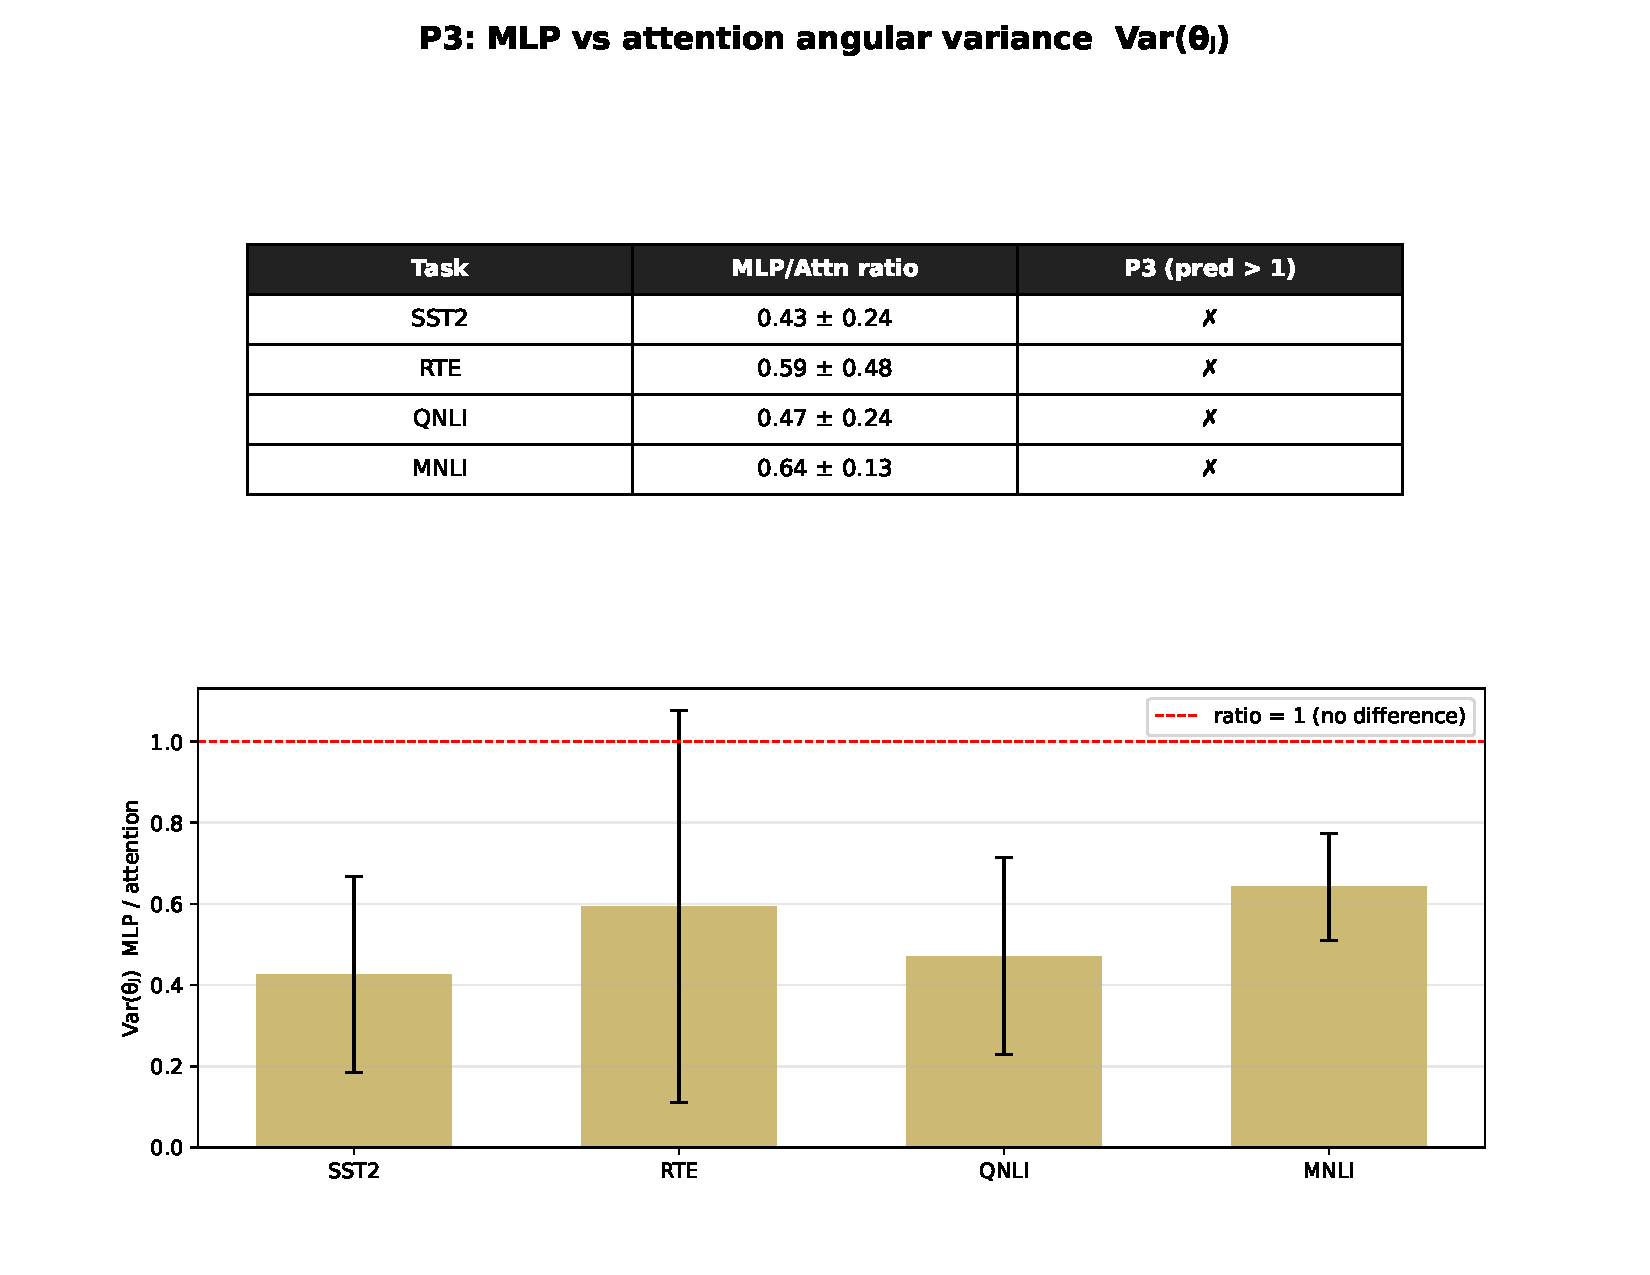
\includegraphics[width=\linewidth]{agg_p3.pdf}
\caption{\textbf{P3: MLP/attention angular-variance ratio per task.} All four tasks
fall \emph{below} the ratio $=1$ line (red dashed), contradicting the predicted
$>1.5$. The ratio increases with task difficulty (SST-2 $<$ QNLI $<$ MNLI), trending
toward---but not reaching---the prediction.}
\label{fig:p3}
\end{figure}

\begin{figure}[t]
\centering
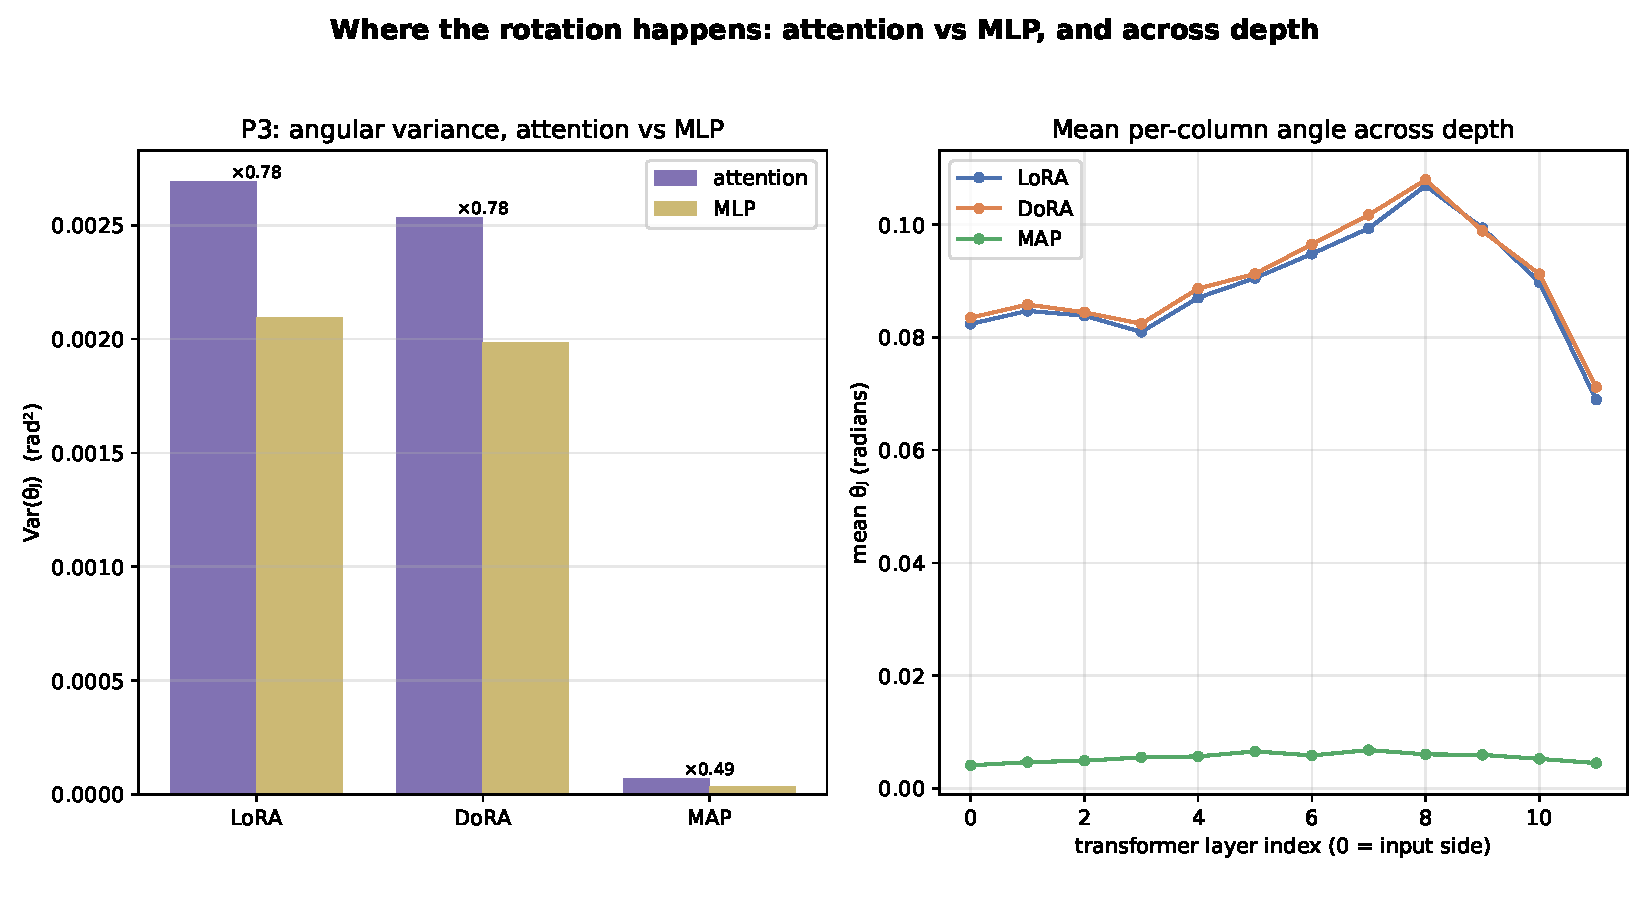
\includegraphics[width=\linewidth]{mnli_layers.pdf}
\caption{\textbf{MNLI: attention vs.\ MLP and depth.} (Left) Per-column angular
variance by layer type (MLP/attention ratios annotated, all $<1$). (Right) Mean
$\theta_j$ across depth---a U-/hump shape peaking in the upper-middle layers for
LoRA/DoRA; MAP stays flat near zero.}
\label{fig:mnli-layers}
\end{figure}

\subsection{Summary of Empirical Findings}
Across four GLUE tasks (36 runs, full data), the results split cleanly into a
\emph{validated geometric and quantitative core} and \emph{two correlational
predictions that do not hold in the form tested}.

\noindent\textbf{Confirmed.}
\begin{enumerate}[leftmargin=*,itemsep=1pt]
\item \textbf{Theorem~\ref{thm:comparison}} (sum-vs-average identity): exact to machine
precision ($2.2\times10^{-16}$) in unit-column form, and linear with $R^2=0.995$,
slope $0.89$ across all $2592$ measured layers in the raw-flattening form.
\item \textbf{Theorem~\ref{thm:nonasym}} (KL bracket): $0/2592$ violations; the exact
$C_{\mathrm{dir}}$ hugs the lower bound since $A_d(\kappa)\ll1$.
\item \textbf{Prediction~P4}: the asymptotic approximation overestimates the
directional KL by $77\times$ ($d{=}768$) to $307\times$ ($d{=}3072$); this tightening
is decisive.
\item \textbf{Non-vacuous bounds}: all $36$ McAllester bound values are $<1$ and tight
on the large tasks (e.g.\ MNLI bound ref.\ $0.131$ vs.\ test error $0.122$)---a direct
consequence of large $n$ and the $A_d(\kappa)$ correction.
\end{enumerate}

\noindent\textbf{Not supported (as tested).}
\begin{enumerate}[leftmargin=*,itemsep=1pt]
\item \textbf{P1} ($\widehat{\Cdir}$ predicts test error): the naive cross-task
Spearman \emph{reverses} ($\rho_S=-0.37$). This is driven by an expressiveness/fitting
confound---MAP rotates little (low $\widehat{\Cdir}$) yet fits worse (high error),
while LoRA/DoRA rotate more and fit better---so absolute test error, rather than the
train-controlled \emph{generalization gap} the bound concerns, anti-correlates with
complexity in this underfitting-limited regime.
\item \textbf{P3} (MLP $>$ attention angular variance): not supported---attention
shows higher variance on all four tasks (ratio $0.43$--$0.64<1$), though the ratio
rises monotonically with task difficulty, trending toward the prediction.
\end{enumerate}

\noindent Accuracy is matched for LoRA/DoRA with MAP a few points behind, and most
full-data tasks are dense ($s/d\to1$) with only tiny RTE sparse, so both regimes of
Theorem~\ref{thm:dora-sparse} appear across tasks. \textbf{Overall:} the theory's
geometric and quantitative machinery is empirically validated and produces tight,
non-vacuous bounds; the two correlational predictions require confound-corrected
re-tests (within-task, training-error-controlled gap for P1; domain-shift tasks for
P3), which we identify as the immediate next experiments.
\section{Discussion}

\subsection{Practical Guidance: When to Use DoRA vs.\ MAP}
The key observable is the effective sparsity ratio $s/d$. \emph{Use DoRA when $s/d$
is small}: column-wise decomposition concentrates complexity where the update
actually occurs and distinguishes a sparse, localized update from a globally diffuse
one. \emph{Use MAP when $s/d\approx1$ and $\mathrm{Var}(\theta_j)$ is low}: when
nearly all columns rotate by approximately the same angle, the global rotation
captures the shared structure in a single degree of freedom. The variance of
$\{\theta_j\}$ serves as a cheap diagnostic computable after a short fine-tuning run.
Our SST-2 pilot ($s/d\approx0.4$, heavy-tailed $\theta_j$) places this setting on the
DoRA-favored side, consistent with DoRA's competitive accuracy.

\subsection{Calibrating $\kappa$}
The concentration $\kappa$ encodes confidence that the pretrained directions are
meaningful for the target task: large $\kappa$ (in-domain) prevents needless drift;
small $\kappa$ (large domain shift) allows free rotation at the cost of a looser
bound. The PAC-Bayes bound provides a computable oracle: the $\kappa$ minimizing the
right-hand side of Theorem~\ref{thm:dora-bound} on held-out data is the theoretically
optimal choice, a principled alternative to grid search.

\subsection{Limitations and Extensions}
The mean-field assumption (A1) ignores inter-column correlations; relaxing it
requires matrix-variate distributions with harder KL computations. The
equal-concentration assumption (A4) ignores layer heterogeneity; per-column $\kappa_j$
is a straightforward extension. As with most PAC-Bayes analyses the bounds may be
numerically vacuous for large models without Monte-Carlo estimation of the partition
function. Empirically, our results are currently a single-task pilot; the
disconfirming P3 observation in particular must be re-evaluated across all six GLUE
tasks and on a domain-shift setting before drawing conclusions about layer-specific
guidance.

\section{Conclusion}
We developed a PAC-Bayesian framework for weight-decomposed PEFT, giving the first
principled comparison between column-wise (DoRA) and global (MAP) adaptation from a
generalization perspective. The Angular Complexity Comparison
(Theorem~\ref{thm:comparison}) and the DoRA-advantage theorem
(Theorem~\ref{thm:dora-sparse}) show the two methods occupy complementary regimes,
the Gibbs posterior derivation justifies cosine regularization, and the
non-asymptotic vMF KL bounds extend the theory beyond the high-concentration limit.
Our first empirical study operationalizes the directional-complexity estimator on
RoBERTa-base/SST-2, confirming the central sum-vs-average identity and the
sparse-update regime while honestly flagging a task-dependent tension with the
attention-vs-MLP prediction. Completing the six-task GLUE sweep is the immediate next
step toward a full validation.

\begin{thebibliography}{99}
\bibitem{dora} S.-Y.\ Liu et al., ``DoRA: Weight-Decomposed Low-Rank Adaptation,''
\emph{arXiv:2402.09353}, 2024.
\bibitem{map} C.\ Si et al., ``MAP: Revisiting Weight Decomposition for Low-Rank
Adaptation,'' \emph{arXiv:2505.23094}, 2025.
\bibitem{lora} E.\ J.\ Hu et al., ``LoRA: Low-Rank Adaptation of Large Language
Models,'' \emph{arXiv:2106.09685}, 2021.
\bibitem{mcallester} D.\ A.\ McAllester, ``Some PAC-Bayesian Theorems,''
\emph{Machine Learning}, 37(3):355--363, 1999.
\bibitem{catoni} O.\ Catoni, \emph{PAC-Bayesian Supervised Classification}, IMS
Lecture Notes, 2007.
\bibitem{pactuning} Y.\ Liu et al., ``PAC-tuning: Fine-tuning Pretrained Language
Models with PAC-Bayes,'' \emph{arXiv:2310.17588}, 2023.
\bibitem{sparse} W.\ Song et al., ``Sparse is Enough in Fine-tuning Pre-trained Large
Language Models,'' \emph{ICML}, 2024.
\bibitem{adalora} Q.\ Zhang et al., ``AdaLoRA: Adaptive Budget Allocation for
Parameter-Efficient Fine-Tuning,'' \emph{ICLR}, 2023.
\bibitem{tanwar} E.\ Tanwar et al., ``Understanding the Effects of Domain Finetuning
on LLMs,'' \emph{arXiv:2510.09359}, 2025.
\bibitem{roberta} Y.\ Liu et al., ``RoBERTa: A Robustly Optimized BERT Pretraining
Approach,'' \emph{arXiv:1907.11692}, 2019.
\end{thebibliography}

\end{document}
